卷积码将k个信息比特编码成n个比特,适合以串行形式传。其编码器一般表示为$(n,k,m)$的形式,其中k为每次输入到卷积编码器的比特数,n为每次输入k位比特后输出的编码长度,m为编码存储长度。

本次实验中,我们使用的是$(2,1,3)$卷积编码,每输入一个信息比特,编码产生两位比特的输出,其框图如图.\ref{fig:encoder}所示。

\begin{figure}[htb]
\centering
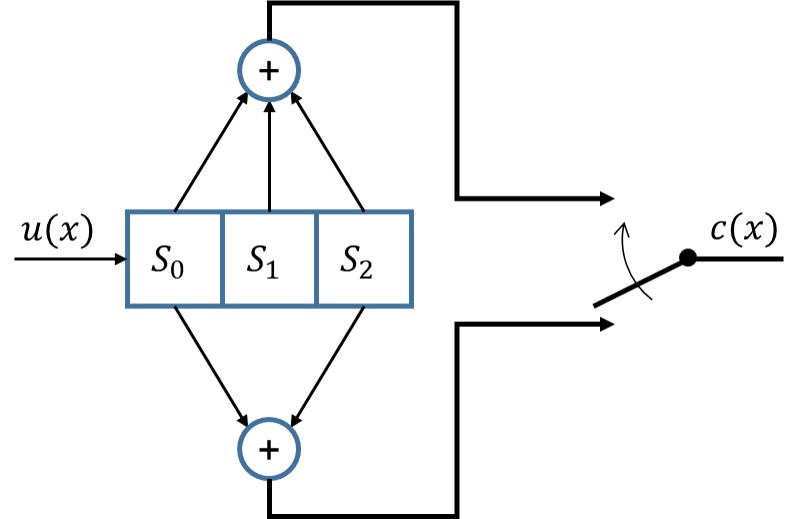
\includegraphics[width=0.4\textwidth]{images//encoder.jpg}
\caption{\label{fig:encoder}(2,1,3)编码器}
\end{figure}

编码器的输入端口信号为:
\begin{itemize}
\item clk\quad        输入控制时钟
\item clk2\quad       输出控制时钟
\item data\_in\quad    编码数据输入
\item reset\quad    重置位
\end{itemize}
其中clk2用于对编码后数据进行控制输出,由于我们采用$(2,1,3)$编码器,故而clk2的频率是clk的两倍。

编码器的输出端口信号为:
\begin{itemize}
\item code\_out\quad        编码数据输出
\item valid\quad       编码有效标志位
\item valid\_wave\quad    编码有效信息流
\end{itemize}
由于我们设计了交织和调制解调模块,需要保证信号同步才能使系统正确工作,所以我们设计了valid以及valid\_wave这两个控制信号来进行各模块间的信号同步。

我们还定义了一个寄存器数组state,用于存储之前时刻的输入。由框图可知,code\_out和state的关系可以表示为:\\
\quad\quad\quad code\_out[0]~=~data\_in + state[0] + state[1]\\
\quad\quad\quad code\_out[1]~=~data\_in + state[1]

每次输入一位比特,编码两位输出,并将valid置为有效。当reset有效时,state清空,并将valid置为无效。

仿真波形如图.\ref{fig:fangzhen}所示。其中data\_send为原始序列,code\_send为编码后序列;二者对应的时钟分别为clk\_div2和clk。从图中可以看出,data\_send每字符占用周期是code\_send两倍。下面用Python检验了一下输出结果,如图
.\ref{fig:PythonSimu},可见我们的编码是正确的。

\begin{figure}[htb]
\centering

\includegraphics[width=0.9\textwidth]{images//encoder_simulation.jpg}
\caption{\label{fig:fangzhen}(2,1,3)编码器仿真波形}
\end{figure}

\begin{figure}[htb]
\centering
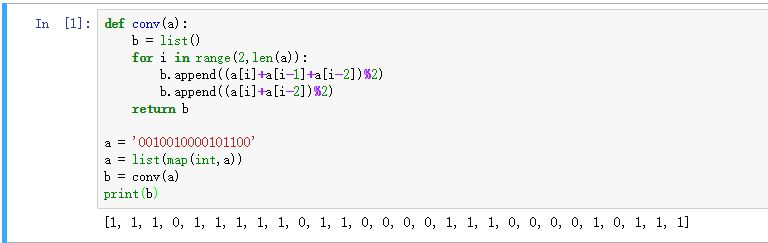
\includegraphics[width=0.8\textwidth]{images//python_simulation.jpg}
\caption{\label{fig:PythonSimu}(2,1,3)编码器输出}
\end{figure}

